\chapter{De energie van reacties: verbranding en bindingsenergieën}\label{ch:g11:reaction-energy}

Breek het zegeltje van een handwarmer en een minuut later is hij te heet
om lang vast te houden; knijp in een koelkompres en het koelt een
verstuikte enkel; een stadsbus rijdt de hele dag op waterstof en laat
alleen waterdamp achter. Chemische omzettingen maken niet alleen van de
ene stof een andere: ze geven energie af, of nemen die op. Waar komt die
energie vandaan, en hoeveel kan een \omterm{def:g4:what-a-fire-needs:fuel}{brandstof} er leveren?

\begin{recall}
Bij een \omterm{def:g8:combustion-and-fuels:complete}{volledige verbranding} verbrandt een \omterm{def:g4:what-a-fire-needs:fuel}{brandstof} die uit koolstof en
waterstof bestaat in zuurstof tot koolstofdioxide en water
(\cref{ch:g8:combustion-and-fuels}). Een \omterm{def:g10:lewis-and-shape:covalent-bond}{covalente binding} is een
gedeeld elektronenpaar; \omterm{def:g10:lewis-and-shape:lewis-structure}{lewisstructuren} laten elke binding van een
\omterm{def:g7:atoms-and-molecules:molecule}{molecuul} zien (\cref{ch:g10:lewis-and-shape}). Een \omterm{def:g10:the-mole:amount}{hoeveelheid stof} tel
je in \omterm{def:g10:the-mole:amount}{mol} (\cref{ch:g10:the-mole}).
\end{recall}

\begin{omfigure}
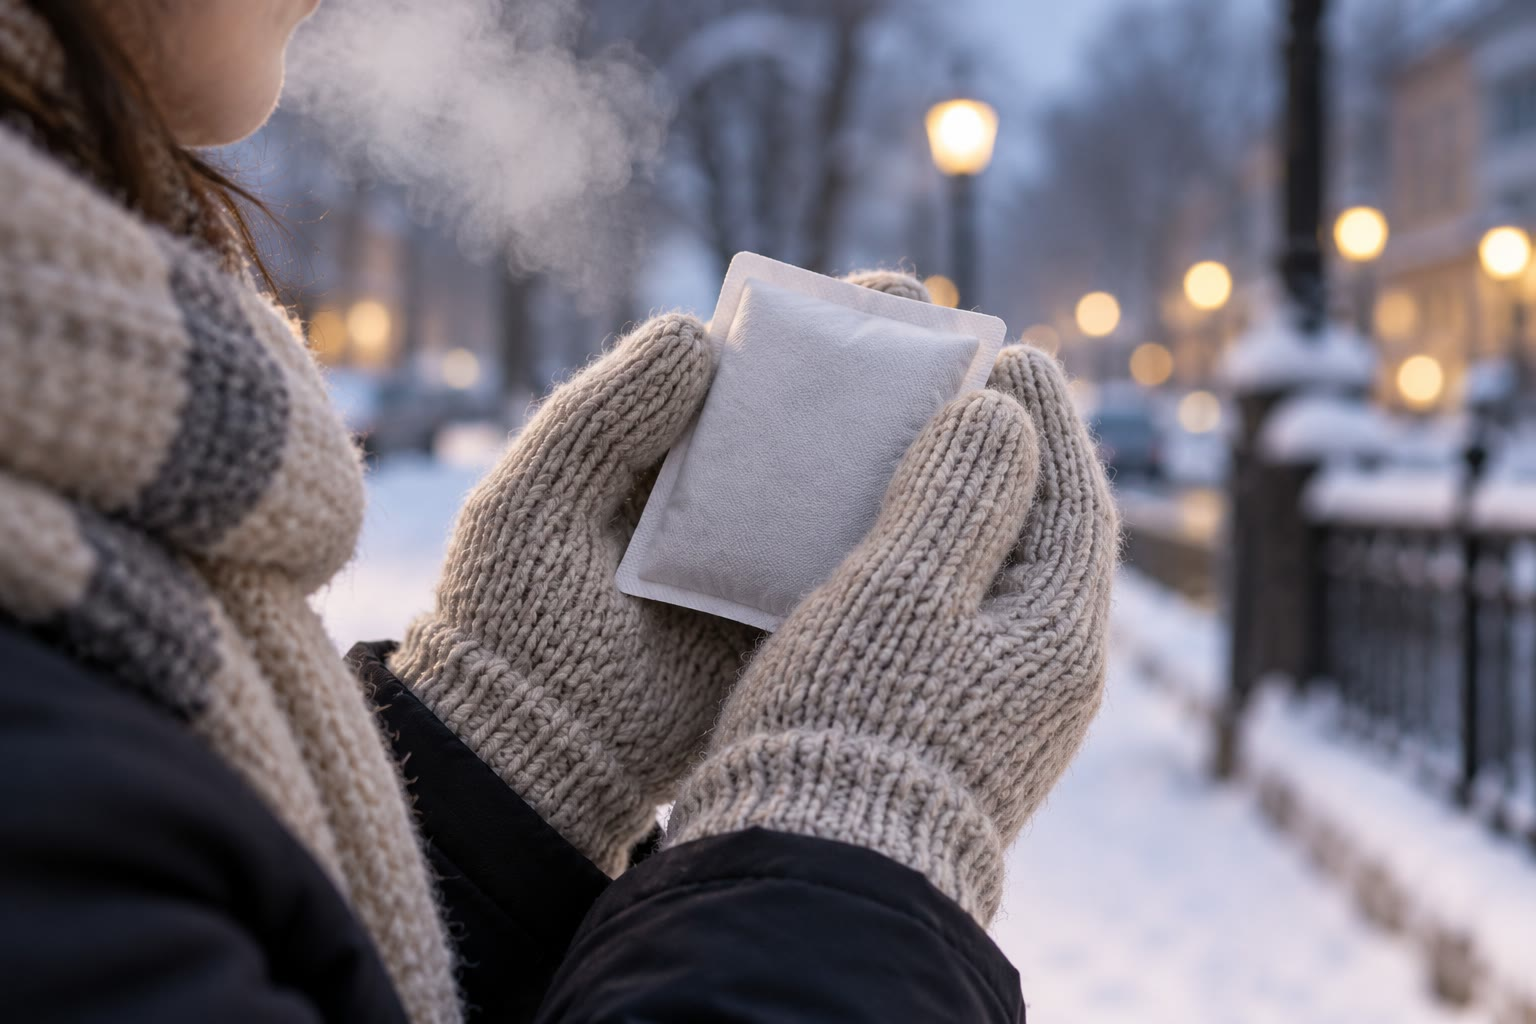
\includegraphics[width=0.45\linewidth]{images/book1/ai/g11-hand-warmers.jpg}

{\small Een handwarmer: een reactie in het zakje geeft warmte af.}
\end{omfigure}

\section{Exotherme en endotherme omzettingen}

\begin{definition}[Exotherm, endotherm]\label{def:g11:reaction-energy:exothermic}
Een omzetting is \emph{exotherm}\index{exotherm} als ze energie afgeeft
aan haar omgeving, meestal als warmte: de omgeving warmt op. Ze is
\emph{endotherm}\index{endotherm} als ze energie opneemt uit haar
omgeving: die koelt af, of de omzetting moet verwarmd worden om door te
gaan.
\end{definition}

\begin{example}[Warm en koud]\label{ex:g11:reaction-energy:packs}
\omterm{def:g4:what-a-fire-needs:burning}{Verbrandingen} zijn \omterm{def:g11:reaction-energy:exothermic}{exotherm}, en dat geldt ook voor de langzame reactie
van ijzerpoeder met de zuurstof uit de \omterm{def:g4:air-a-mixture-of-gases:air}{lucht} in een handwarmer. Het
\omterm{def:g2:mixing-and-dissolving:dissolve}{oplossen} van ammoniumnitraat in water, dat in koelkompressen gebruikt
wordt, is \omterm{def:g11:reaction-energy:exothermic}{endotherm}; dat geldt ook voor de ontleding van kalksteen in
ongebluste kalk en koolstofdioxide, die alleen in een zeer hete kalkoven
plaatsvindt.
\end{example}

\begin{omfigure}
\begin{tikzpicture}[font=\small]
  \begin{scope}
    \draw[->] (0,0) -- (0,3.2) node[above] {energie};
    \draw[very thick, omDef] (0.5,2.5) -- (2.3,2.5) node[right, text=black] {beginstoffen};
    \draw[very thick, omProp] (0.5,0.8) -- (2.3,0.8) node[right, text=black] {reactieproducten};
    \draw[->, thick, omThm] (1.4,2.45) -- (1.4,0.85);
    \node[omThm, anchor=west, align=left] at (1.5,1.65) {energie\\ afgegeven};
    \node[anchor=north] at (1.6,-0.15) {\textbf{exotherm}};
  \end{scope}
  \begin{scope}[xshift=6cm]
    \draw[->] (0,0) -- (0,3.2) node[above] {energie};
    \draw[very thick, omDef] (0.5,0.8) -- (2.3,0.8) node[right, text=black] {beginstoffen};
    \draw[very thick, omProp] (0.5,2.5) -- (2.3,2.5) node[right, text=black] {reactieproducten};
    \draw[->, thick, omDef] (1.4,0.85) -- (1.4,2.45);
    \node[omDef, anchor=west, align=left] at (1.5,1.65) {energie\\ opgenomen};
    \node[anchor=north] at (1.6,-0.15) {\textbf{endotherm}};
  \end{scope}
\end{tikzpicture}

{\small Energiediagrammen. Bij een \omterm{def:g11:reaction-energy:exothermic}{exotherme} reactie bevatten de
\omterm{def:g7:chemical-reactions:reactant}{reactieproducten} minder energie dan de \omterm{def:g7:chemical-reactions:reactant}{beginstoffen}, en het verschil komt
vrij; bij een \omterm{def:g11:reaction-energy:exothermic}{endotherme} reactie bevatten ze meer, en dat verschil moet
worden toegevoerd.}
\end{omfigure}

\section{De energie die een verbranding afgeeft}

\begin{definition}[Molaire verbrandingsenergie]\label{def:g11:reaction-energy:combustion-energy}
De \emph{molaire verbrandingsenergie}\index{molaire verbrandingsenergie}
$E_c$ van een \omterm{def:g4:what-a-fire-needs:fuel}{brandstof} is de energie die vrijkomt bij de \omterm{def:g8:combustion-and-fuels:complete}{volledige
verbranding} van één \omterm{def:g10:the-mole:amount}{mol} ervan, in \si{kJ/mol}, waarbij het gevormde
water vloeibaar is.
\end{definition}

\begin{proposition}[Energie die $n$ mol afgeeft]\label{prop:g11:reaction-energy:n-moles}
% ledger: dch:CH4
De \omterm{def:g8:combustion-and-fuels:complete}{volledige verbranding} van een hoeveelheid $n$ \omterm{def:g4:what-a-fire-needs:fuel}{brandstof} geeft de
energie $Q = n \times E_c$ af. Voor methaan is $E_c = \qty{890.7}{kJ/mol}$:
de \omterm{def:g4:what-a-fire-needs:burning}{verbranding} van \qty{1.00}{mol} (\qty{16.0}{g}) ervan geeft ongeveer
\qty{891}{kJ} af.
\end{proposition}

\begin{proof}
Elke \omterm{def:g10:the-mole:amount}{mol} \omterm{def:g4:what-a-fire-needs:fuel}{brandstof} die verbrandt, geeft $E_c$ af; $n$ \omterm{def:g10:the-mole:amount}{mol} geven $n$ keer
zoveel.
\end{proof}

\begin{inthelab}[Water verwarmen met een spiritusbrander]
% ledger: cp:water
Een spiritusbrander met ethanol wordt gewogen en daarna aangestoken onder
een \omterm{def:g9:periodic-table-first-look:metal}{metalen} blikje met \qty{200}{g} water, met een thermometer erin. Als
het water \qty{25}{\celsius} warmer is geworden, wordt de vlam gedoofd en
de brander opnieuw gewogen: hij is \qty{1.50}{g} ethanol kwijtgeraakt. De
energie die het water heeft opgenomen, bereken je met de natuurkundige
formule $Q = m\, c\, \Delta\theta$,
waarin $c = \qty{4.18}{J/(g.\celsius)}$ de soortelijke warmte van water
is. Ze ligt ver onder de energie die de ethanol zou kunnen afgeven: veel
van de warmte verwarmt de \omterm{def:g4:air-a-mixture-of-gases:air}{lucht}, het blikje en de brander, en een deel
van de ethanol verbrandt onvolledig.
\end{inthelab}

\begin{omfigure}
\begin{tikzpicture}[font=\small]
  % spirit burner
  \fill[black!8, draw=black!60] (-0.6,0) rectangle (0.6,0.7);
  \fill[cyan!15] (-0.55,0.05) rectangle (0.55,0.45);
  \fill[black!40] (-0.06,0.7) rectangle (0.06,0.95);
  \fill[orange!70!yellow] (0,0.95) .. controls (-0.25,1.25) and (-0.1,1.6) .. (0,1.85)
    .. controls (0.1,1.6) and (0.25,1.25) .. (0,0.95);
  \fill[yellow!40] (0,1.0) .. controls (-0.1,1.2) and (-0.05,1.4) .. (0,1.5)
    .. controls (0.05,1.4) and (0.1,1.2) .. (0,1.0);
  % tripod and can
  \draw[black!60, line width=1pt] (-1.1,0) -- (-0.9,2.1) (1.1,0) -- (0.9,2.1);
  \draw[black!60, line width=1.2pt] (-1.1,2.1) -- (1.1,2.1);
  \fill[black!15, draw=black!60] (-0.8,2.1) rectangle (0.8,3.7);
  \fill[omWater] (-0.75,2.15) rectangle (0.75,3.3);
  % thermometer
  \pic at (0.35,2.35) {thermometer};
  \draw[omProp, thick, <-] (0.6,0.35) -- (2.0,0.35) node[right, text=black]
    {spiritusbrander (ethanol)};
  \draw[omProp, thick, <-] (0.8,2.9) -- (2.0,2.9) node[right, text=black]
    {blikje: \qty{200}{g} water};
  \draw[omProp, thick, <-] (0.45,5.0) -- (2.0,5.0) node[right, text=black]
    {thermometer};
\end{tikzpicture}

{\small De energie meten die een \omterm{def:g4:what-a-fire-needs:fuel}{brandstof} levert: een spiritusbrander
verwarmt een blikje water, waarvan de temperatuurstijging gemeten wordt.}
\end{omfigure}


\begin{example}[De spiritusbrander in getallen]\label{ex:g11:reaction-energy:burner}
% ledger: cp:water, dch:C2H5OH, aw:C, aw:H, aw:O
Het water nam $Q = 200 \times 4.18 \times 25 = \qty{2.09e4}{J}$ op,
dat is \qty{20.9}{kJ}. De verbrande ethanol, \qty{1.50}{g}, is
$1.50 / 46.0 = \qty{0.0326}{mol}$; met $E_c = \qty{1367.6}{kJ/mol}$
had die $0.0326 \times 1367.6 = \qty{44.6}{kJ}$ kunnen afgeven. Slechts
$20.9 / 44.6 \approx \qty{47}{\percent}$ daarvan kwam bij het water terecht.
\end{example}

\section{Bindingsenergieën}

\begin{definition}[Bindingsenergie]\label{def:g11:reaction-energy:bond-energy}
De \emph{bindingsenergie}\index{bindingsenergie} van een \omterm{def:g10:lewis-and-shape:covalent-bond}{covalente
binding} is de energie die nodig is om één \omterm{def:g10:the-mole:amount}{mol} van zulke bindingen te
verbreken, waarbij de \omterm{def:g7:atoms-and-molecules:molecule}{moleculen} en \omterm{def:g7:atoms-and-molecules:atom}{atomen} gasvormig zijn. Tabellen geven
gemiddelde waarden, gemeten over veel \omterm{def:g7:atoms-and-molecules:molecule}{moleculen}, in \si{kJ/mol}.
\end{definition}

\begin{omfigure}
\small
% ledger: be:H-H, be:C-H, be:N-H, be:O-H, be:H-Cl, be:C-C, be:CC-double, be:C-O, be:CO-double, be:NN-triple, be:OO-double, be:Cl-Cl
\begin{tabular}{lr@{\qquad}lr@{\qquad}lr}
\hline
binding & \si{kJ/mol} & binding & \si{kJ/mol} & binding & \si{kJ/mol} \\
\hline
\ce{H-H} & 436 & \ce{C-C} & 345 & \ce{O=O} & 498 \\
\ce{C-H} & 415 & \ce{C=C} & 611 & \ce{N#N} & 946 \\
\ce{N-H} & 390 & \ce{C-O} & 350 & \ce{Cl-Cl} & 243 \\
\ce{O-H} & 464 & \ce{C=O} & 741 & \ce{H-Cl} & 432 \\
\hline
\end{tabular}\par\medskip


{\small Gemiddelde bindingsenergieën. Het verbreken van een binding kost
altijd energie; bij het vormen ervan komt dezelfde energie weer vrij.}
\end{omfigure}

\begin{omfigure}
\begin{tikzpicture}[font=\small, x=1cm, y=0.0015cm]
  \draw[->] (0,-850) -- (0,2900) node[above] {energie (\si{kJ})};
  \draw[very thick, black!60] (0.4,2656) -- (3.9,2656);
  \node[anchor=west] at (4.0,2656) {losse atomen: \ce{C + 4H + 4O}};
  \draw[very thick, omDef] (0.4,0) -- (3.9,0);
  \node[anchor=west] at (4.0,0) {\ce{CH4 + 2O2}};
  \draw[very thick, omProp] (0.4,-682) -- (3.9,-682);
  \node[anchor=west] at (4.0,-682) {\ce{CO2 + 2H2O}};
  \draw[->, thick, omDef] (1.0,30) -- (1.0,2626);
  \node[omDef, anchor=west, align=left] at (1.05,1500) {verbreek 4 \ce{C-H}\\ en 2 \ce{O=O}:\\ $+\qty{2656}{kJ}$};
  \draw[->, thick, omProp] (3.4,2626) -- (3.4,-652);
  \node[omProp, anchor=west, align=left] at (3.45,1200) {vorm 2 \ce{C=O}\\ en 4 \ce{O-H}:\\ $-\qty{3338}{kJ}$};
  \draw[<->, omThm, thick] (0.6,-10) -- (0.6,-672);
  \node[omThm, anchor=west] at (0.65,-341) {$E_r \approx \qty{-682}{kJ}$};
\end{tikzpicture}


{\small De \omterm{def:g4:what-a-fire-needs:burning}{verbranding} van methaan als twee denkbeeldige stappen, met
gemiddelde bindingsenergieën: eerst elke binding verbreken, dan de
nieuwe vormen. De schatting, \qty{-682}{kJ} per \omterm{def:g10:the-mole:amount}{mol} methaan, is
\omterm{def:g11:reaction-energy:exothermic}{exotherm}.}
\end{omfigure}

\begin{proposition}[Een reactie-energie schatten]\label{prop:g11:reaction-energy:estimate}
Voor een reactie tussen gassen is de opgenomen energie $E_r$ (negatief
als er energie vrijkomt) bij benadering
\[
  E_r \approx \sum E(\text{verbroken bindingen}) - \sum E(\text{gevormde bindingen}) .
\]
Als $E_r < 0$, komt er bij het vormen van de nieuwe bindingen meer
energie vrij dan er nodig is om de oude te verbreken: de reactie is
\omterm{def:g11:reaction-energy:exothermic}{exotherm}.
\end{proposition}

\begin{proof}
Stel je de reactie in twee stappen voor: elke binding van de
\omterm{def:g7:chemical-reactions:reactant}{beginstoffen} wordt verbroken, wat de eerste som kost en losse \omterm{def:g7:atoms-and-molecules:atom}{atomen}
oplevert; daarna vormen zich de bindingen van de \omterm{def:g7:chemical-reactions:reactant}{reactieproducten}, wat
de tweede som teruggeeft. Het resultaat is maar een schatting, omdat
tabellen gemiddelden over veel \omterm{def:g7:atoms-and-molecules:molecule}{moleculen} geven.
\end{proof}

\begin{method}[Een reactie-energie schatten uit bindingsenergieën]\label{met:g11:reaction-energy:bonds}
\begin{enumerate}
  \item Schrijf de \omterm{def:g8:balanced-equations:equation}{kloppende reactievergelijking} op en de \omterm{def:g10:lewis-and-shape:lewis-structure}{lewisstructuur}
        van elk \omterm{def:g7:atoms-and-molecules:molecule}{molecuul}.
  \item Tel, met de \omterm{def:g8:balanced-equations:coefficient}{coëfficiënten}, de bindingen van elke soort die in de
        \omterm{def:g7:chemical-reactions:reactant}{beginstoffen} verbroken en in de \omterm{def:g7:chemical-reactions:reactant}{reactieproducten} gevormd worden.
  \item Tel de energieën van de verbroken bindingen op, en trek die van
        de gevormde bindingen ervan af.
  \item Concludeer: een negatief resultaat betekent een \omterm{def:g11:reaction-energy:exothermic}{exotherme}
        reactie.
\end{enumerate}
\end{method}

\begin{example}[Waterstof en chloor]\label{ex:g11:reaction-energy:hcl}
% ledger: be:H-H, be:Cl-Cl, be:H-Cl
Voor \ce{H2 + Cl2 -> 2HCl}: één \ce{H-H} en één \ce{Cl-Cl} verbroken,
$436 + 243 = \qty{679}{kJ}$; twee \ce{H-Cl} gevormd, $2 \times 432 =
\qty{864}{kJ}$. Dus $E_r \approx 679 - 864 = \qty{-185}{kJ}$ per \omterm{def:g10:the-mole:amount}{mol}
reactie: \omterm{def:g11:reaction-energy:exothermic}{exotherm}.
\end{example}


\begin{remark}[Schatting en meting]\label{rem:g11:reaction-energy:compare}
% ledger: dch:CH4
De gemeten energie die vrijkomt bij de \omterm{def:g4:what-a-fire-needs:burning}{verbranding} van één \omterm{def:g10:the-mole:amount}{mol} methaan is
\qty{890.7}{kJ}, meer dan de schatting. Er zijn drie redenen: de
\ce{C=O}-bindingen van koolstofdioxide zijn sterker dan de gemiddelde
\ce{C=O} uit de tabel; de gemeten waarde geldt voor vloeibaar water, en
bij het condenseren van de waterdamp komt nog meer energie vrij; en
gemiddelde bindingsenergieën zijn nu eenmaal gemiddelden. De methode van
de bindingsenergieën geeft het teken en de orde van grootte, niet de
precieze waarde.
\end{remark}

\section{Brandstoffen vergelijken}

\begin{omfigure}
\begin{tikzpicture}
\begin{axis}[xbar, width=0.78\linewidth, height=5.4cm, xmin=0, xmax=160,
    xlabel={energie die vrijkomt per verbrande kilogram (\si{MJ/kg})},
    symbolic y coords={ethanol, octane, propane, methane, hydrogen},
    ytick=data, yticklabels={ethanol, octaan, propaan, methaan, waterstof},
    bar width=10pt, nodes near coords,
    nodes near coords style={font=\footnotesize, /pgf/number format/fixed,
      /pgf/number format/precision=1, /pgf/number format/fixed zerofill},
    tick label style={font=\small}, label style={font=\small},
    axis lines*=left, xmajorgrids, grid style={gray!20}, enlarge y limits=0.15]
  % ledger: dch:C2H5OH, dfh:C8H18, dfh:CO2, dfh:H2O-l, dch:C3H8, dch:CH4 (per kg with the book's molar masses)
  \addplot[fill=omProp!55, draw=omProp] coordinates {(29.7,ethanol) (48.0,octane)
    (50.4,propane) (55.7,methane) (142.9,hydrogen)};
\end{axis}
\end{tikzpicture}

{\small De energie die vrijkomt bij de \omterm{def:g8:combustion-and-fuels:complete}{volledige verbranding} van één
kilogram van vijf \omterm{def:g4:what-a-fire-needs:fuel}{brandstoffen} (gevormd water vloeibaar). Waterstof
levert per kilogram verreweg het meest; ethanol, dat al gedeeltelijk
``verbrand'' is (het bevat zuurstof), het minst.}
\end{omfigure}

\begin{example}[Koolstofdioxide per megajoule]\label{ex:g11:reaction-energy:co2}
% ledger: dch:CH4, dch:C2H5OH
De \omterm{def:g4:what-a-fire-needs:burning}{verbranding} van één \omterm{def:g10:the-mole:amount}{mol} methaan geeft \qty{890.7}{kJ} en één \omterm{def:g10:the-mole:amount}{mol}
koolstofdioxide, \qty{44.0}{g}. Voor één megajoule, \qty{1000}{kJ},
komt er dus $44.0 \times 1000 / 890.7 = \qty{49.4}{g}$ koolstofdioxide
vrij. Ethanol, met twee \omterm{def:g10:the-mole:amount}{mol} koolstofdioxide per \qty{1367.6}{kJ}, geeft
$88.0 \times 1000 / 1367.6 = \qty{64.3}{g}$ per megajoule. Waterstof
geeft niets: zijn enige \omterm{def:g7:chemical-reactions:reactant}{reactieproduct} is water.
\end{example}

\begin{omfigure}
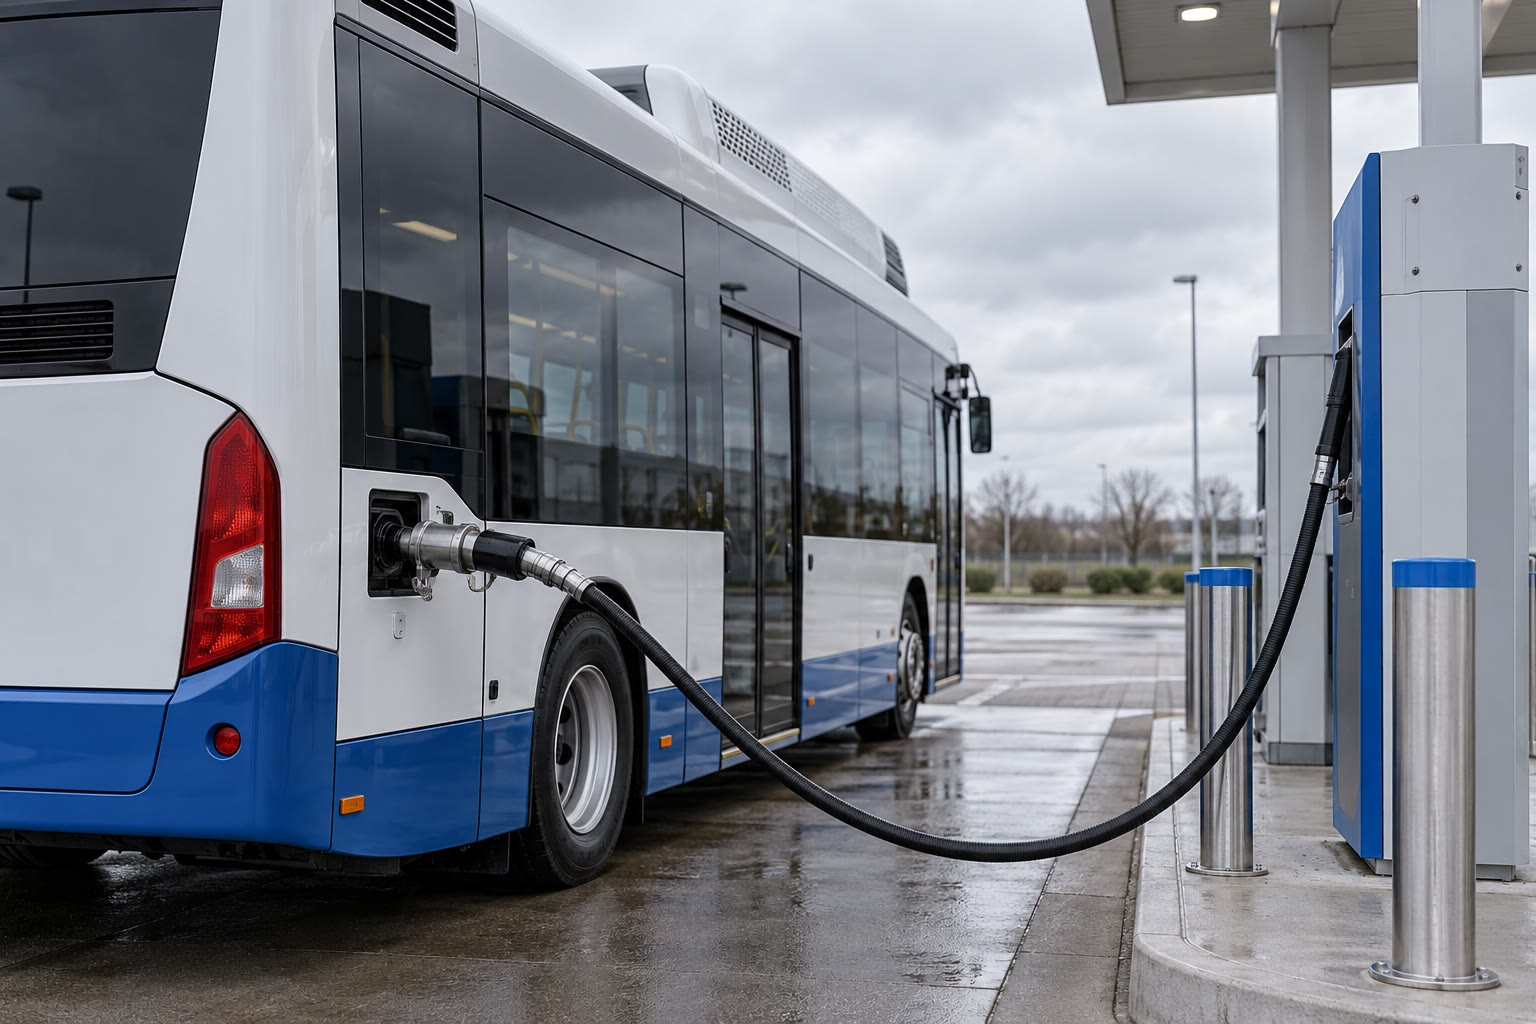
\includegraphics[width=0.5\linewidth]{images/book1/ai/g11-hydrogen-bus.jpg}

{\small Een bus bij een waterstoftankstation: zijn \omterm{def:g4:what-a-fire-needs:fuel}{brandstof} levert
alleen water op.}
\end{omfigure}

\begin{safety}{\ghs[0.82cm]{GHS02}\ghs[0.82cm]{GHS07}}
% ledger: ghs:ethanol
Ethanol is zeer licht ontvlambaar en irriterend voor de ogen. Een
spiritusbrander wordt gevuld ver van elke vlam, nooit bijgevuld zolang
hij heet is, en door de docent gebruikt op een hittebestendige onderlaag.
\end{safety}

\section{Oefeningen}


\begin{exercise}[$\star$]\label{exo:g11:reaction-energy:1}
\omterm{def:g11:reaction-energy:exothermic}{Exotherm} of \omterm{def:g11:reaction-energy:exothermic}{endotherm}: hout dat brandt; ijs dat smelt; een koelkompres
waarin geknepen wordt; een handwarmer die warm wordt; een groen blad dat
in het zonlicht suiker maakt?
\end{exercise}

\begin{exercise}[$\star$]\label{exo:g11:reaction-energy:2}
% ledger: dch:CH4
Hoeveel energie komt er vrij bij de \omterm{def:g8:combustion-and-fuels:complete}{volledige verbranding} van
\qty{3.0}{mol} methaan?
\end{exercise}

\begin{exercise}[$\star$]\label{exo:g11:reaction-energy:3}
Wat bevat in het energiediagram van een \omterm{def:g11:reaction-energy:exothermic}{exotherme} reactie meer energie,
de \omterm{def:g7:chemical-reactions:reactant}{beginstoffen} of de \omterm{def:g7:chemical-reactions:reactant}{reactieproducten}? Waar blijft het verschil?
\end{exercise}

\begin{exercise}[$\star$]\label{exo:g11:reaction-energy:4}
% ledger: dch:C2H5OH
Hoeveel energie komt er vrij bij de \omterm{def:g8:combustion-and-fuels:complete}{volledige verbranding} van
\qty{100}{g} ethanol?
\end{exercise}

\begin{exercise}[$\star$]\label{exo:g11:reaction-energy:5}
Wat is een \omterm{def:g11:reaction-energy:bond-energy}{bindingsenergie}? Waarom kost het verbreken van een binding
altijd energie?
\end{exercise}

\begin{exercise}[$\star\star$]\label{exo:g11:reaction-energy:6}
Schat met bindingsenergieën de energie van de reactie
\ce{2H2 + O2 -> 2H2O}, alles gasvormig. Is ze \omterm{def:g11:reaction-energy:exothermic}{exotherm}?
\end{exercise}

\begin{exercise}[$\star\star$]\label{exo:g11:reaction-energy:7}
Schat de energie van de \omterm{def:g4:what-a-fire-needs:burning}{verbranding} van ethanol, \ce{C2H5OH + 3O2 ->
2CO2 + 3H2O}, met bindingsenergieën (teken eerst de \omterm{def:g10:lewis-and-shape:lewis-structure}{lewisstructuur} van
ethanol), en vergelijk met de gemeten \qty{1367.6}{kJ/mol}.
\end{exercise}

\begin{exercise}[$\star\star$]\label{exo:g11:reaction-energy:8}
% ledger: dch:C3H8, dch:CH4
Bereken de energie die vrijkomt per kilogram propaan
(\qty{2219.2}{kJ/mol}) en per kilogram methaan. Vergelijk met het
staafdiagram.
\end{exercise}

\begin{exercise}[$\star\star$]\label{exo:g11:reaction-energy:9}
% ledger: cp:water, dch:CH4
Een gasfornuis verwarmt \qty{1.50}{L} water (\qty{1500}{g}) van
\qty{15}{\celsius} tot \qty{100}{\celsius}. Hoeveel energie neemt het
water op? Welke massa methaan wordt er verbrand als alle energie bij het
water terechtkomt? En als maar de helft dat doet?
\end{exercise}

\begin{exercise}[$\star\star$]\label{exo:g11:reaction-energy:10}
Zet met het staafdiagram de \omterm{def:g4:what-a-fire-needs:fuel}{brandstoffen} op volgorde van energie per
kilogram. Welke massa waterstof levert evenveel energie als
\qty{1.0}{kg} octaan?
\end{exercise}

\begin{exercise}[$\star\star$]\label{exo:g11:reaction-energy:11}
Schat de energie van \ce{N2 + 3H2 -> 2NH3}, alles gasvormig. \omterm{def:g11:reaction-energy:exothermic}{Exotherm} of
\omterm{def:g11:reaction-energy:exothermic}{endotherm}?
\end{exercise}

\begin{exercise}[$\star\star\star$]\label{exo:g11:reaction-energy:12}
% ledger: cp:water, dch:C2H5OH
Bij een proef met een spiritusbrander wordt \qty{250}{g} water
\qty{20}{\celsius} warmer terwijl er \qty{1.20}{g} ethanol verbrandt.
Bereken de energie die het water opneemt, de energie die de ethanol zou
kunnen afgeven, en het rendement van de verwarming. Noem drie oorzaken
van de verliezen.
\end{exercise}

\begin{exercise}[$\star\star\star$]\label{exo:g11:reaction-energy:13}
% ledger: dfh:C8H18, dfh:CO2, dfh:H2O-l, dch:C3H8
Octaan geeft \qty{5470}{kJ/mol} af en propaan \qty{2219.2}{kJ/mol}.
Schrijf hun verbrandingsvergelijkingen op en bereken de massa
koolstofdioxide die elk per megajoule uitstoot. Vergelijk met methaan,
\qty{49.4}{g}.
\end{exercise}

\begin{exercise}[$\star\star\star$]\label{exo:g11:reaction-energy:14}
Voor zowel methaan als ethanol is de schatting met bindingsenergieën
kleiner dan de gemeten energie die vrijkomt. Geef de redenen, en leg uit
waarom de schatting toch nuttig is.
\end{exercise}

\begin{exercise}[$\star\star\star$]\label{exo:g11:reaction-energy:15}
Schat de energie van \ce{2H2O -> 2H2 + O2}, alles gasvormig. Waarom moet
er energie worden toegevoerd (bijvoorbeeld als elektriciteit) om
waterstof uit water te maken? Leg uit waarom waterstof een manier heet om
energie \emph{op te slaan}, en niet een energiebron.
\end{exercise}

\section{Probleem: Welke brandstof voor de stadsbus?}

\begin{problem}[{Weekendprobleem --- methaan, ethanol, octaan of waterstof:
welke levert de meeste energie per kilogram, en hoeveel koolstofdioxide
per megajoule?}]
\label{pb:g11:reaction-energy:1}
% ledger: dch:CH4, dch:C2H5OH, dfh:C8H18, dfh:CO2, dfh:H2O-l, be:C-H, be:OO-double, be:CO-double, be:O-H
Een stad vergelijkt vier \omterm{def:g4:what-a-fire-needs:fuel}{brandstoffen} voor haar bussen: methaan
(aardgas), ethanol, octaan (voor benzine) en waterstof. De energieën die
vrijkomen bij de \omterm{def:g8:combustion-and-fuels:complete}{volledige verbranding} van één \omterm{def:g10:the-mole:amount}{mol} zijn: methaan
\qty{890.7}{kJ}, ethanol \qty{1367.6}{kJ}, octaan \qty{5470}{kJ},
waterstof \qty{285.8}{kJ}, waarbij het gevormde water vloeibaar is.

\medskip
\noindent\textbf{Deel I --- Verbrandingsvergelijkingen.}
\begin{enumerate}
  \item Schrijf de vergelijking op van de \omterm{def:g8:combustion-and-fuels:complete}{volledige verbranding} van
        methaan.
  \item Van ethanol, \ce{C2H6O}.
  \item Van octaan, \ce{C8H18}.
  \item Van waterstof.
  \item Welke \omterm{def:g4:what-a-fire-needs:fuel}{brandstof} stoot geen koolstofdioxide uit?
\end{enumerate}

\medskip
\noindent\textbf{Deel II --- Energie per kilogram.}
\begin{enumerate}[resume]
  \item Bereken de \omterm{def:g10:the-mole:molar-mass}{molaire massa's} van de vier \omterm{def:g4:what-a-fire-needs:fuel}{brandstoffen}.
  \item Bereken voor elk de energie die per kilogram vrijkomt, in
        \si{MJ/kg}.
  \item Zet de \omterm{def:g4:what-a-fire-needs:fuel}{brandstoffen} op volgorde.
  \item Waterstof wint met afstand. Waarom is het toch lastig om het in
        een bus mee te nemen? (Denk aan zijn fase bij kamertemperatuur.)
\end{enumerate}

\medskip
\noindent\textbf{Deel III --- Schatten met bindingsenergieën.}
\begin{enumerate}[resume]
  \item Teken de \omterm{def:g10:lewis-and-shape:lewis-structure}{lewisstructuren} van de \omterm{def:g7:atoms-and-molecules:molecule}{moleculen} bij de \omterm{def:g4:what-a-fire-needs:burning}{verbranding} van
        methaan, en tel de verbroken en de gevormde bindingen.
  \item Bereken de energie die nodig is om de bindingen te verbreken.
  \item Bereken de energie die vrijkomt bij het vormen van de nieuwe
        bindingen.
  \item Leid de schatting van $E_r$ af, en vergelijk met de gemeten
        waarde: wat is het relatieve verschil?
  \item Geef twee redenen voor het verschil.
\end{enumerate}

\medskip
\noindent\textbf{Deel IV --- Koolstofdioxide per megajoule.}
\begin{enumerate}[resume]
  \item Welke hoeveelheid methaan moet er \omterm{def:g4:what-a-fire-needs:burning}{verbranden} om \qty{1}{MJ} af te
        geven?
  \item Welke massa koolstofdioxide komt daarbij vrij?
  \item Dezelfde vraag voor ethanol en octaan.
  \item Welke koolstofhoudende \omterm{def:g4:what-a-fire-needs:fuel}{brandstof} stoot voor dezelfde energie de
        minste koolstofdioxide uit? Waarom (vergelijk de aantallen C- en
        \omterm{def:g7:atoms-and-molecules:atom}{H-atomen})?
  \item Waterstof stoot bij \omterm{def:g4:what-a-fire-needs:burning}{verbranding} niets uit. Waar hangt zijn
        werkelijke voordeel voor het klimaat van af?
  \item Geef het eindantwoord: welke massa koolstofdioxide stoot methaan
        per megajoule uit?
\end{enumerate}
\end{problem}
